
In order to understand the motivations, limitations and behaviour of the experiment we need to know about a few key concepts in fluid dynamics.

\subsection{Navier Stokes}


\subsection{Reynold's Number}
The Reynolds number (Re) is a dimensionless number describing the ratio of inertial forces to viscous forces in a flow. This is not a very strict definition, but suffices to explain that the Reynolds number can be used to characterize the so called flow regime of a system. 

The two major flow regimes are Laminar flow, where viscous forces dominate over inertial forces, and the turbulent regime where inertial forces dominate. The area where neither is significantly larger is referred to as transitional flow, which may show either chaotic of laminar behaviour. 

A rough characterization of laminar and chaotic flow can be seen in figure \ref{fig:laminar_flow}

\begin{figure}
\centering
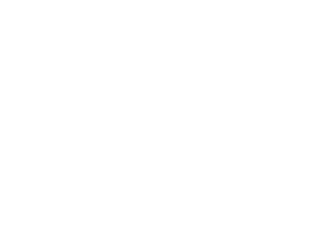
\includegraphics[width=\textwidth]{figures/theory/laminarFlow.pdf}
\caption{This shows the principal difference between laminar and turbulent flow}
\label{fig:laminar_flow}
\end{figure}

The Reynolds number (Re) is defined as \cite{introfluid}

\begin{equation}\label{eq:reynolds}
Re = \frac{U L \rho}{\mu}
\end{equation}

where $U$ is the characteristic velocity, $L$ is the characteristic length, $\rho$ is the density and $\mu$ is the dynamic viscosity. 

As the Reynolds number is a ratio, a flow is predicted to be laminar if $Re << 1$ which is the primary concern in this thesis.

\subsection{Stokes Drag and Stokes's law}
The drag force $F_D$ exerted by a fluid on a spherical particle for $Re << 1$ is found using the so called Stokes's law \cite{introfluid2}

\begin{equation}
F_D = 6\pi \mu R v
\end{equation}

where $v$ is the velocity of the sphere relative to the fluid, $\mu$ is the dynamic viscosity and $R$ is the radius of the sphere. To find the terminal velocity of the sphere we equate this with the gravitational force $F_G$ acting on the sphere

\begin{equation}
F_G = \Delta \rho g\cdot \frac{4\pi R^3}{3}
\end{equation}

where $\Delta \rho$ is the difference in density and $g$ is the specific gravity we find that the terminal velocity of a sinking (or floating) sphere is

\begin{equation}\label{eq:fallingSphere}
v_s = \frac{2}{9} \frac{\Delta \rho}{\mu} g R^2
\end{equation}



%\subsection{Shear}
%
%\subsection{P\'{e}clet Number}
%The p\'{}clet number describes the ratio of thermal noise to other stuff. I really don't know anything about the piclet number.
